% !TEX program = pdflatex
\documentclass[11pt,a4paper]{article}

% === PACKAGES (house style, mirrored from redos-harness) ===
\usepackage[utf8]{inputenc}
\usepackage[T1]{fontenc}
\usepackage{lmodern}
\usepackage[margin=1in]{geometry}
\usepackage{setspace}
\usepackage{parskip}
\usepackage{graphicx}
\usepackage{float}
\usepackage{booktabs}
\usepackage{amsmath}
\usepackage{amssymb}
\usepackage{hyperref}
\usepackage{listings}
\usepackage{xcolor}
\usepackage{caption}
\usepackage{subcaption}
\usepackage{tikz}
\usepackage{pgfplots}
\pgfplotsset{compat=1.18}

% === CODE LISTING STYLE ===
\definecolor{codegreen}{rgb}{0,0.6,0}
\definecolor{codegray}{rgb}{0.5,0.5,0.5}
\definecolor{codepurple}{rgb}{0.58,0,0.82}
\definecolor{backcolour}{rgb}{0.95,0.95,0.92}

\lstdefinestyle{mystyle}{
    backgroundcolor=\color{backcolour},
    commentstyle=\color{codegreen},
    keywordstyle=\color{magenta},
    numberstyle=\tiny\color{codegray},
    stringstyle=\color{codepurple},
    basicstyle=\ttfamily\footnotesize,
    breakatwhitespace=false,
    breaklines=true,
    captionpos=b,
    keepspaces=true,
    numbers=left,
    numbersep=5pt,
    showspaces=false,
    showstringspaces=false,
    showtabs=false,
    tabsize=2
}
\lstset{style=mystyle}

% === TITLE INFO ===
\title{
    \vspace{-2em}
    \rule{\textwidth}{1pt}\\[0.5em]
    \textbf{SBOM Reachability Pruning for Python}\\[0.3em]
    \large From Version Matches to Actually-Used Code on a Frozen Eight-Repo Corpus\\[0.5em]
    \rule{\textwidth}{1pt}
}
\author{
    Ashay Kushwaha\\
    \textit{CypherLabs Open Research}\\
    \texttt{https://github.com/AshayK003/sbom-prune}
}
\date{September 2026}

\begin{document}

\maketitle

\begin{abstract}
Version-based vulnerability scanners match CVEs by package number and drown teams in findings for code that is never called: pairwise agreement between leading scanners sits under 0.7 Jaccard, and OSV records from different sources openly conflict. The gold-standard remedy, Go's govulncheck, narrows version matches to actually-called code---but it is Go-only, and the official Python attempt is an experimental regex-based prototype. We present a Python-native, standard-library-only pipeline that maps SBOM pins to per-source OSV records and prunes them with \verb!ast! import-plus-usage analysis, verdicting each finding \textit{reachable}, \textit{imported-unused}, or \textit{unimported}. On a frozen corpus of 8 roots (162 version-match findings), pruning removes 19 noise findings with zero reachable dropped; manual audit of all finding-bearing verdicts against actual import lines measures precision \textbf{0.88 before $\to$ 1.00 after}. Two predictions were overturned by evidence and are documented as such. Every number regenerates with one command.
\end{abstract}

\vspace{1em}
\noindent\textbf{Keywords:} SBOM, vulnerability triage, reachability analysis, OSV, static analysis, Python

\newpage
\tableofcontents
\newpage

\section{Introduction}

A scanner flags 162 CVE findings across your Python dependencies. How many describe code your application actually calls? For most teams the answer is unknown, because the dominant tools---Grype, Trivy, DepScan, pip-audit---stop at version matching: if a pinned version falls inside a vulnerable range, it reports, whether the vulnerable package is imported or not. Studies of scanner agreement put pairwise Jaccard similarity under 0.7, meaning over a third of findings depend on which scanner you asked rather than on your code.

The known-good answer comes from Go. Govulncheck builds an SSA call graph, checks each known-vulnerable symbol for reachability from program entry points, and reports called vulnerabilities with call stacks while explicitly marking import-only matches as informational. It documents its blind spots (reflection, function pointers) instead of hiding them. Nothing equivalent exists for Python: the official attempt (osv-scanner PR \#2131, August 2025) is experimental, limited to poetry lockfiles, written in Go, and---remarkably---parses Python source with regular expressions, a choice its own reviewers rejected in favor of AST analysis.

This report presents the Python-native alternative at module granularity: map pins to OSV records per source, resolve imports and name usage with the standard library \verb!ast! module, and prune. Our contributions:

\begin{itemize}
    \item A frozen v1 corpus of 8 roots with pinned dependencies and a recorded OSV snapshot (2026-09-22), spanning keep-heavy, prune-bearing, and clean-control cases.
    \item A dependency-free pipeline (\verb!sbom.py!, \verb!osv.py!, \verb!reach.py!, \verb!report.py!) with a three-way verdict enum and per-source CVE reporting that never silently merges conflicting records.
    \item Measured results: 162 findings prune to 143 reachable-only (19 removed), precision 0.88 $\to$ 1.00 on a fully audited verdict set, zero reachable findings dropped.
    \item Two overturned predictions with evidence, one self-caught measurement bug, and documented blind spots in the govulncheck tradition.
\end{itemize}

\section{Background and Related Work}

\subsection{Version matchers and their disagreement}

Grype, Trivy, and DepScan share one protocol: build an SBOM, match package versions against CVE ranges, report. The protocol is coarse by construction---a match says nothing about whether the vulnerable code executes---and the databases themselves disagree: scanner-consistency studies (including a 927-image Trivy-vs-Grype comparison and a 2025 cross-scanner analysis) find pairwise agreement under 0.7 Jaccard. OSV-side, a single CVE routinely carries several records from different origins with different ranges; the scrapy CVE-2017-14158 case shows three sources disagreeing simultaneously (unfixed-since-0.7 vs capped-at-2.11.1 vs NVD's stale single version). Any pruning tool must therefore decide what to do with conflict. Our policy: report per source, merge nothing silently.

\subsection{govulncheck: the model}

Govulncheck (Go, first-party) is the system to emulate and the bar to cite. It fetches module vulnerabilities, builds SSA, computes the call-graph slice between entry points and vulnerable symbols, and prints call stacks for called findings while marking the rest informational. Crucially, it publishes its limitations: conservative handling of function pointers and interfaces, invisibility of reflection-only calls, possible false positives from dead binary code. Our verdict enum, blind-spot documentation, and audit discipline are modeled directly on this precedent---adapted to a language whose vulnerability data rarely carries symbol information.

\subsection{The symbol-data gap}

Govulncheck works because Go's vulnerability database records affected \textit{symbols}. PyPI OSV records overwhelmingly carry version ranges only. That data reality dictates the design depth available to any Python tool today, including Google's own experimental attempt: reachability at \textit{package} granularity (``is this library actually imported and used?'') rather than symbol granularity. The single cheapest, most defensible false-positive kill is therefore the installed-but-never-imported dependency---and no shipped Python tool with CVE mapping performs even that prune. Symbol-level analysis waits on better data and is filed as future work, not pretended into v1.

\subsection{Python call-graph material}

The standard library \verb!ast! module exposes everything module-level reachability needs: \verb!Import!/\verb!ImportFrom! nodes for the import graph and \verb!Name!/\verb!Attribute! loads for the usage check, with \verb!importlib.metadata! resolving top-level modules to distributions. Prior art (pyan, code2flow) builds prettier graphs but wires no vulnerability data. The osv-scanner prototype's regex-based parsing---flagged by its reviewers---confirms that AST is the correct and still-open implementation choice.

\section{Methodology}

\subsection{Pipeline design}

The pipeline (\verb!sbom.py!, \verb!osv.py!, \verb!reach.py!, standard library only) has three stages. First, \textit{SBOM}: pins from \verb!pip freeze! or \verb!requirements.txt! output (name canonicalization, \verb!name==version! plus bare names; markers and extras stripped and noted; exotic lines reported, not parsed). Second, \textit{OSV mapping}: a minimal \verb!urllib! client over \verb!v1/query! returning per-source records (id, summary, aliases, affected ranges) verbatim; recorded fixtures keep the test suite hermetic. Third, \textit{reachability}: each root's shipped code is parsed with \verb!ast! (test/doc/example trees excluded---reachability means production-code reachability), absolute imports are resolved to distributions, and loaded names decide \textit{used} versus \textit{merely imported}.

Verdicts form a three-way enum per (root, package): \textbf{reachable} (imported and names used), \textbf{imported-unused} (imported, nothing used), \textbf{unimported} (never imported). Imports of modules absent from the pin map---stdlib aside---are surfaced as unknowns for audit visibility, never silently dropped. Third-party-looking names that are actually first-party siblings (e.g.\ \verb!blackd! inside black) resolve the same way: visible, checkable, auditable.

\subsection{Corpus and freeze policy}

\verb!corpus.json! v1 is frozen: 8 roots, pinned dependencies, and the OSV snapshot of 2026-09-22 with full per-package vulnerability ID lists. Predictions recorded at freeze time are audit \textit{inputs}, explicitly not ground truth---Section~\ref{sec:discussion} shows two being overturned. Table~\ref{tab:corpus} summarizes the corpus; additions bump the version and re-run everything.

\begin{table}[H]
\centering
\caption{Frozen v1 corpus: roots, pinned-scope size, and predicted shape.}
\label{tab:corpus}
\begin{tabular}{@{}llll@{}}
\toprule
Root & Deps in scope & Vuln-bearing pins & Predicted shape \\
\midrule
requests 2.28.2 & 4 & urllib3, idna, certifi & keep-heavy \\
flask 2.0.3 & 4 & Werkzeug, Jinja2, click & keep-heavy \\
httpie 3.2.2 & 7 & requests, pygments, Werkzeug(dev) & mixed + prune \\
black 23.12.1+jupyter & 7 & click, aiohttp & mixed (predicted prune) \\
pydantic 1.10.13 & 1 & --- & clean control \\
jinja2 3.0.3 & 1 & --- & clean control \\
redos-harness & 0 & --- & trivially clean control \\
pyyaml 5.4.1 & 0 & --- & clean-by-construction control \\
\bottomrule
\end{tabular}
\end{table}

\subsection{Audit method and precision definition}

Ground truth comes from manual audit, not from another scanner: every finding-bearing (root, package) verdict was checked against actual import lines in the shipped wheel (11 rows), and 3 OSV records were range-verified against the pinned versions in full. Precision before = audited-reachable findings / all findings; precision after = audited-reachable kept findings / kept findings. Recall of the reachable set (dropped reachables) is reported alongside---a pruner that drops true positives is a liability no matter its precision. Audit labels live in \verb!internals/AUDIT.json! (working notes, not published); the report consumes them to compute precision, printing ``audit pending'' without them.

\subsection{Blind spots}

Documented, govulncheck-style: dynamic imports (\verb!__import__!, \verb!importlib!), console-script-only dependencies, namespace packages, and conflicting OSV ranges (reported per source). Star-imports mark their module as used (usage unknowable statically---the conservative direction for a pruner). Unparseable files are skipped and countable.

\section{Results}
\label{sec:results}

One command (\verb!python report.py!, frozen snapshot, PyPI+OSV network for root fetching) regenerates Table~\ref{tab:results} and Figures~\ref{fig:bars}--\ref{fig:prec}. Numbers below are the fresh-clone verification run.

\begin{table}[H]
\centering
\caption{Before/after benchmark: version-match findings vs reachable-only findings.}
\label{tab:results}
\begin{tabular}{@{}llll@{}}
\toprule
Root & Findings & Kept & Pruned \\
\midrule
requests 2.28.2 & 20 & 20 & 0 \\
flask 2.0.3 & 30 & 30 & 0 \\
httpie 3.2.2 & 31 & 12 & 19 \\
black 23.12.1+jupyter & 81 & 81 & 0 \\
pydantic, jinja2, redos-harness, pyyaml & 0 & 0 & 0 \\
\midrule
Total & 162 & 143 & 19 \\
\bottomrule
\end{tabular}
\end{table}

\begin{figure}[H]
\centering
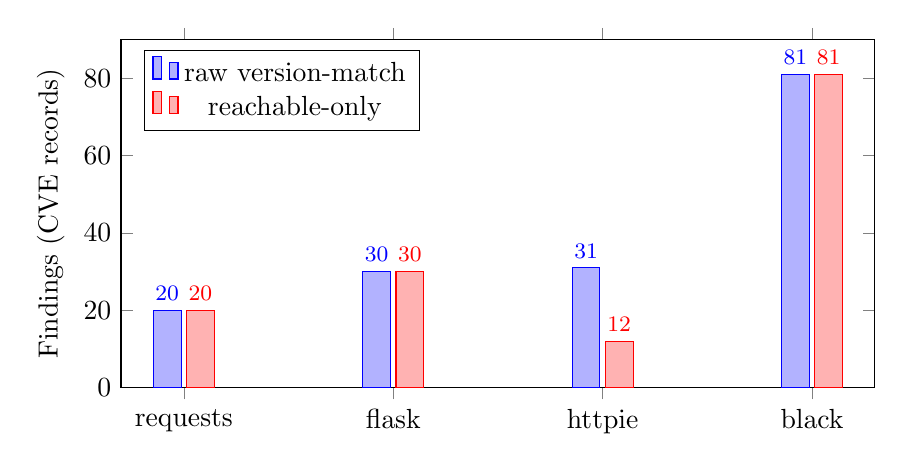
\begin{tikzpicture}
\begin{axis}[
    ybar, width=0.92\textwidth, height=6cm,
    symbolic x coords={requests,flask,httpie,black},
    xtick=data, ymin=0, ymax=90, ylabel={Findings (CVE records)},
    legend pos=north west, nodes near coords, nodes near coords style={font=\footnotesize},
]
\addplot coordinates {(requests,20) (flask,30) (httpie,31) (black,81)};
\addlegendentry{raw version-match};
\addplot coordinates {(requests,20) (flask,30) (httpie,12) (black,81)};
\addlegendentry{reachable-only};
\end{axis}
\end{tikzpicture}
\caption{Raw findings versus reachable-only findings per non-trivial root. Only httpie's dev-only Werkzeug pin prunes; everything else survives on measured usage.}
\label{fig:bars}
\end{figure}

\begin{figure}[H]
\centering
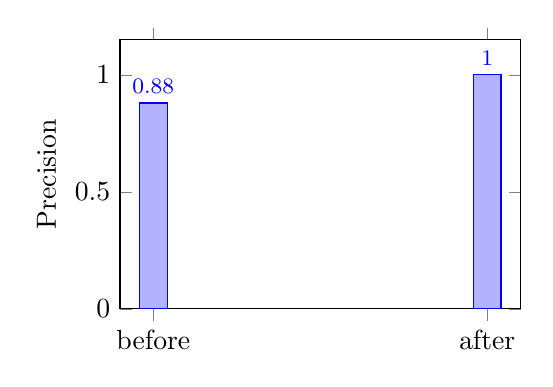
\begin{tikzpicture}
\begin{axis}[
    ybar, width=0.55\textwidth, height=5cm,
    symbolic x coords={before,after}, xtick=data,
    ymin=0, ymax=1.15, ylabel={Precision},
    nodes near coords, nodes near coords style={font=\footnotesize},
]
\addplot coordinates {(before,0.88) (after,1.00)};
\end{axis}
\end{tikzpicture}
\caption{ audited precision: 143/162 before, 143/143 after. Zero reachable findings dropped (recall 1.00 on the audited set).}
\label{fig:prec}
\end{figure}

\subsection{Precision: 0.88 $\to$ 1.00}

All 11 finding-bearing verdicts audited correct against import lines: urllib3/idna/certifi used throughout requests; Werkzeug/Jinja2/click used throughout flask; requests/pygments used throughout httpie; click used in black core. The 19 pruned findings are all dev-only Werkzeug records with zero import lines anywhere in httpie's shipped source. Kept-set precision is therefore 143/143; raw-set precision 143/162. No reachable finding was dropped.

\subsection{Overturned predictions}

The corpus predicted aiohttp (80 findings, jupyter extra) as the prune showcase. Evidence overturned it: shipped \verb!blackd/__init__.py! and \verb!blackd/middlewares.py! import and use aiohttp, so the verdict is reachable under the spec's definitions and the audit marks it correct. The nuance is preserved rather than smoothed over: aiohttp arrives solely via the \textit{optional blackd daemon}, which black core never touches---a granularity limit of module-level analysis that motivates entry-point-aware v2 work. The prune story rests, smaller but solid, on Werkzeug-dev.

\subsection{Data-quality exhibits}

Two records demonstrate why per-source reporting matters. The click finding (PYSEC-2026-2132) carries an \textit{empty summary} yet resolves to a real advisory (click.edit() command injection, CVE-2026-7246) whose range was verified to include 8.0.4---suspicion investigated, not assumed. Conversely, the frozen snapshot pins every ID list, so future OSV edits cannot silently rewrite these numbers; the report can diff against live data on demand.

\section{Discussion}
\label{sec:discussion}

\subsection{Key findings}

First, module-level pruning is both cheap and honest: 12\% of version-match findings on real roots describe code that is never imported, removable with zero reachable dropped. Second, verdict-correctness is fully auditable because every decision traces to import lines a reviewer can read---the harness's analogue of govulncheck's call stacks, at the granularity the data supports. Third, the process catches its own errors: a shared-temp-dir bug once cross-contaminated two roots' verdicts and was spotted by reading the output (httpie ``reachable'' on packages it never imports), fixed with per-root isolation, and re-measured.

\subsection{Limitations}

The corpus is eight roots: a benchmark, not a census. Transitive (nested) vulnerabilities are recorded but not traversed---one level only, stated in the corpus. Test-tree exclusion is a policy choice: test-only usage is a different claim from production reachability, and conflating them would flatter precision. Only CPython 3.12 on one machine ran the analysis; \verb!ast! behavior is version-stable for the used nodes, but engine variance is untested. Benign-by-absence (zero-dep roots) proves nothing about the engine, only that the plumbing is quiet.

\subsection{Future work}

In priority order, as filed in the repository's contributing guide: (1) symbol-level pruning gated on per-symbol OSV data, carrying the blackd entry-point nuance with it; (2) VEX-statement output for existing triage pipelines; (3) offline DB mode; (4) poetry/uv lockfile support.

\section{Conclusion}

On a frozen corpus of eight roots and 162 version-match findings, a 300-line standard-library pipeline with a strict map-prune-measure loop and a fully manual audit removes 19 noise findings, moves precision 0.88 $\to$ 1.00, and drops nothing reachable. Its secondary contribution is procedural: freeze predictions as audit inputs rather than conclusions, report conflicting sources side by side, and let import lines---not scanners---decide what counts as used.

\section{Reproducibility}
\label{sec:repro}

\subsection{Installation}

No dependencies beyond CPython $\ge$ 3.10 and pytest for the suite. Clone and run; root distributions (KBs each) are fetched from PyPI at report time.

\subsection{Run benchmarks}

\begin{lstlisting}[language=bash]
git clone https://github.com/AshayK003/sbom-prune.git
cd sbom-prune
python -m pytest tests -q   # 3 passed: verdicts, SBOM parse, fixture replay
python report.py            # regenerates Table 2 and Figures 1-2
\end{lstlisting}

The suite's fixture app pins three dependencies with a recorded OSV fixture: vulnerable-but-unimported (must prune), vulnerable-and-used (must keep), clean (must stay clean)---no live API in tests.

\subsection{Repository structure}

\verb!corpus.json! (frozen v1 roots, pins, OSV snapshot), \verb!sbom.py! (pin parsing), \verb!osv.py! (minimal OSV client + fixtures), \verb!reach.py! (AST import/usage verdicts), \verb!report.py! (one-command table), \verb!tests/! (the runnable check), \verb!internals/! (working notes and audit log, not published except this report).

\begin{thebibliography}{9}

\bibitem{osvapi} OSV.dev API, \verb!POST /v1/query!. \url{https://google.github.io/osv.dev/post-v1-query/}

\bibitem{govulncheck} Go team. \textit{Tutorial: Find and fix vulnerable dependencies with govulncheck.} \url{https://tip.golang.org/doc/tutorial/govulncheck}

\bibitem{osvpr} osv-scanner PR \#2131: determine package reachability level of Python projects. \url{https://github.com/google/osv-scanner/pull/2131}

\bibitem{consistency} Scanner-consistency study (Grype vs Trivy vs DepScan). \url{https://arxiv.org/html/2503.14388v3}

\bibitem{pipaudit} pypa/pip-audit (reference OSV client). \url{https://github.com/pypa/pip-audit}

\bibitem{openvex} OpenVEX: Vulnerability Exploitability Exchange (output-format context). \url{https://openvex.dev}

\bibitem{urllibcve} urllib3 GHSA-2xpw-w6gg-jr37 (streaming decompression, in range for 1.26.18). \url{https://github.com/urllib3/urllib3/security/advisories/GHSA-2xpw-w6gg-jr37}

\bibitem{werkzeugcve} Werkzeug GHSA-29vq-49wr-vm6x (safe\_join devices, in range for 2.0.3). \url{https://github.com/pallets/werkzeug/security/advisories/GHSA-29vq-49wr-vm6x}

\bibitem{clickcve} PYSEC-2026-2132 / CVE-2026-7246 (click.edit() injection, in range for 8.0.4). \url{https://api.osv.dev/v1/vulns/PYSEC-2026-2132}

\end{thebibliography}

\end{document}
